\usepackage{cite} 
\usepackage{float}
\usepackage[margin = 1.2in]{geometry} % change the page margins
\usepackage{graphicx} % to use \includegraphics
\usepackage{hyperref} % adding urls using \url
\usepackage[utf8]{inputenc} % makes sure other characters than ASCII can be used
\usepackage{parskip} % makes sure that a line is skipped after every paragraph
\usepackage{tikz} % for graphics, also build front cover using tikz
\usepackage{todonotes} % placing todo notes and summarizing them at start of document

%% Change font to sans-serif
\renewcommand\familydefault{\sfdefault}

%% Folder with figures
\graphicspath {{figure/}}

%% Acronym
\usepackage{acronym} 

\hypersetup{ %setup hyperlinks
    colorlinks,
    citecolor=black,
    filecolor=black,
    linkcolor=black,
    urlcolor=black
}

\setlength{\parindent}{0pt}


%% Front cover

\newcommand{\makeCover}{
	%% Create an empty page for cover.
	\clearpage
	\thispagestyle{empty}

 	%% Building cover
	\begin{tikzpicture}[remember picture,overlay]
		\node (picture) at (current page.center)
		{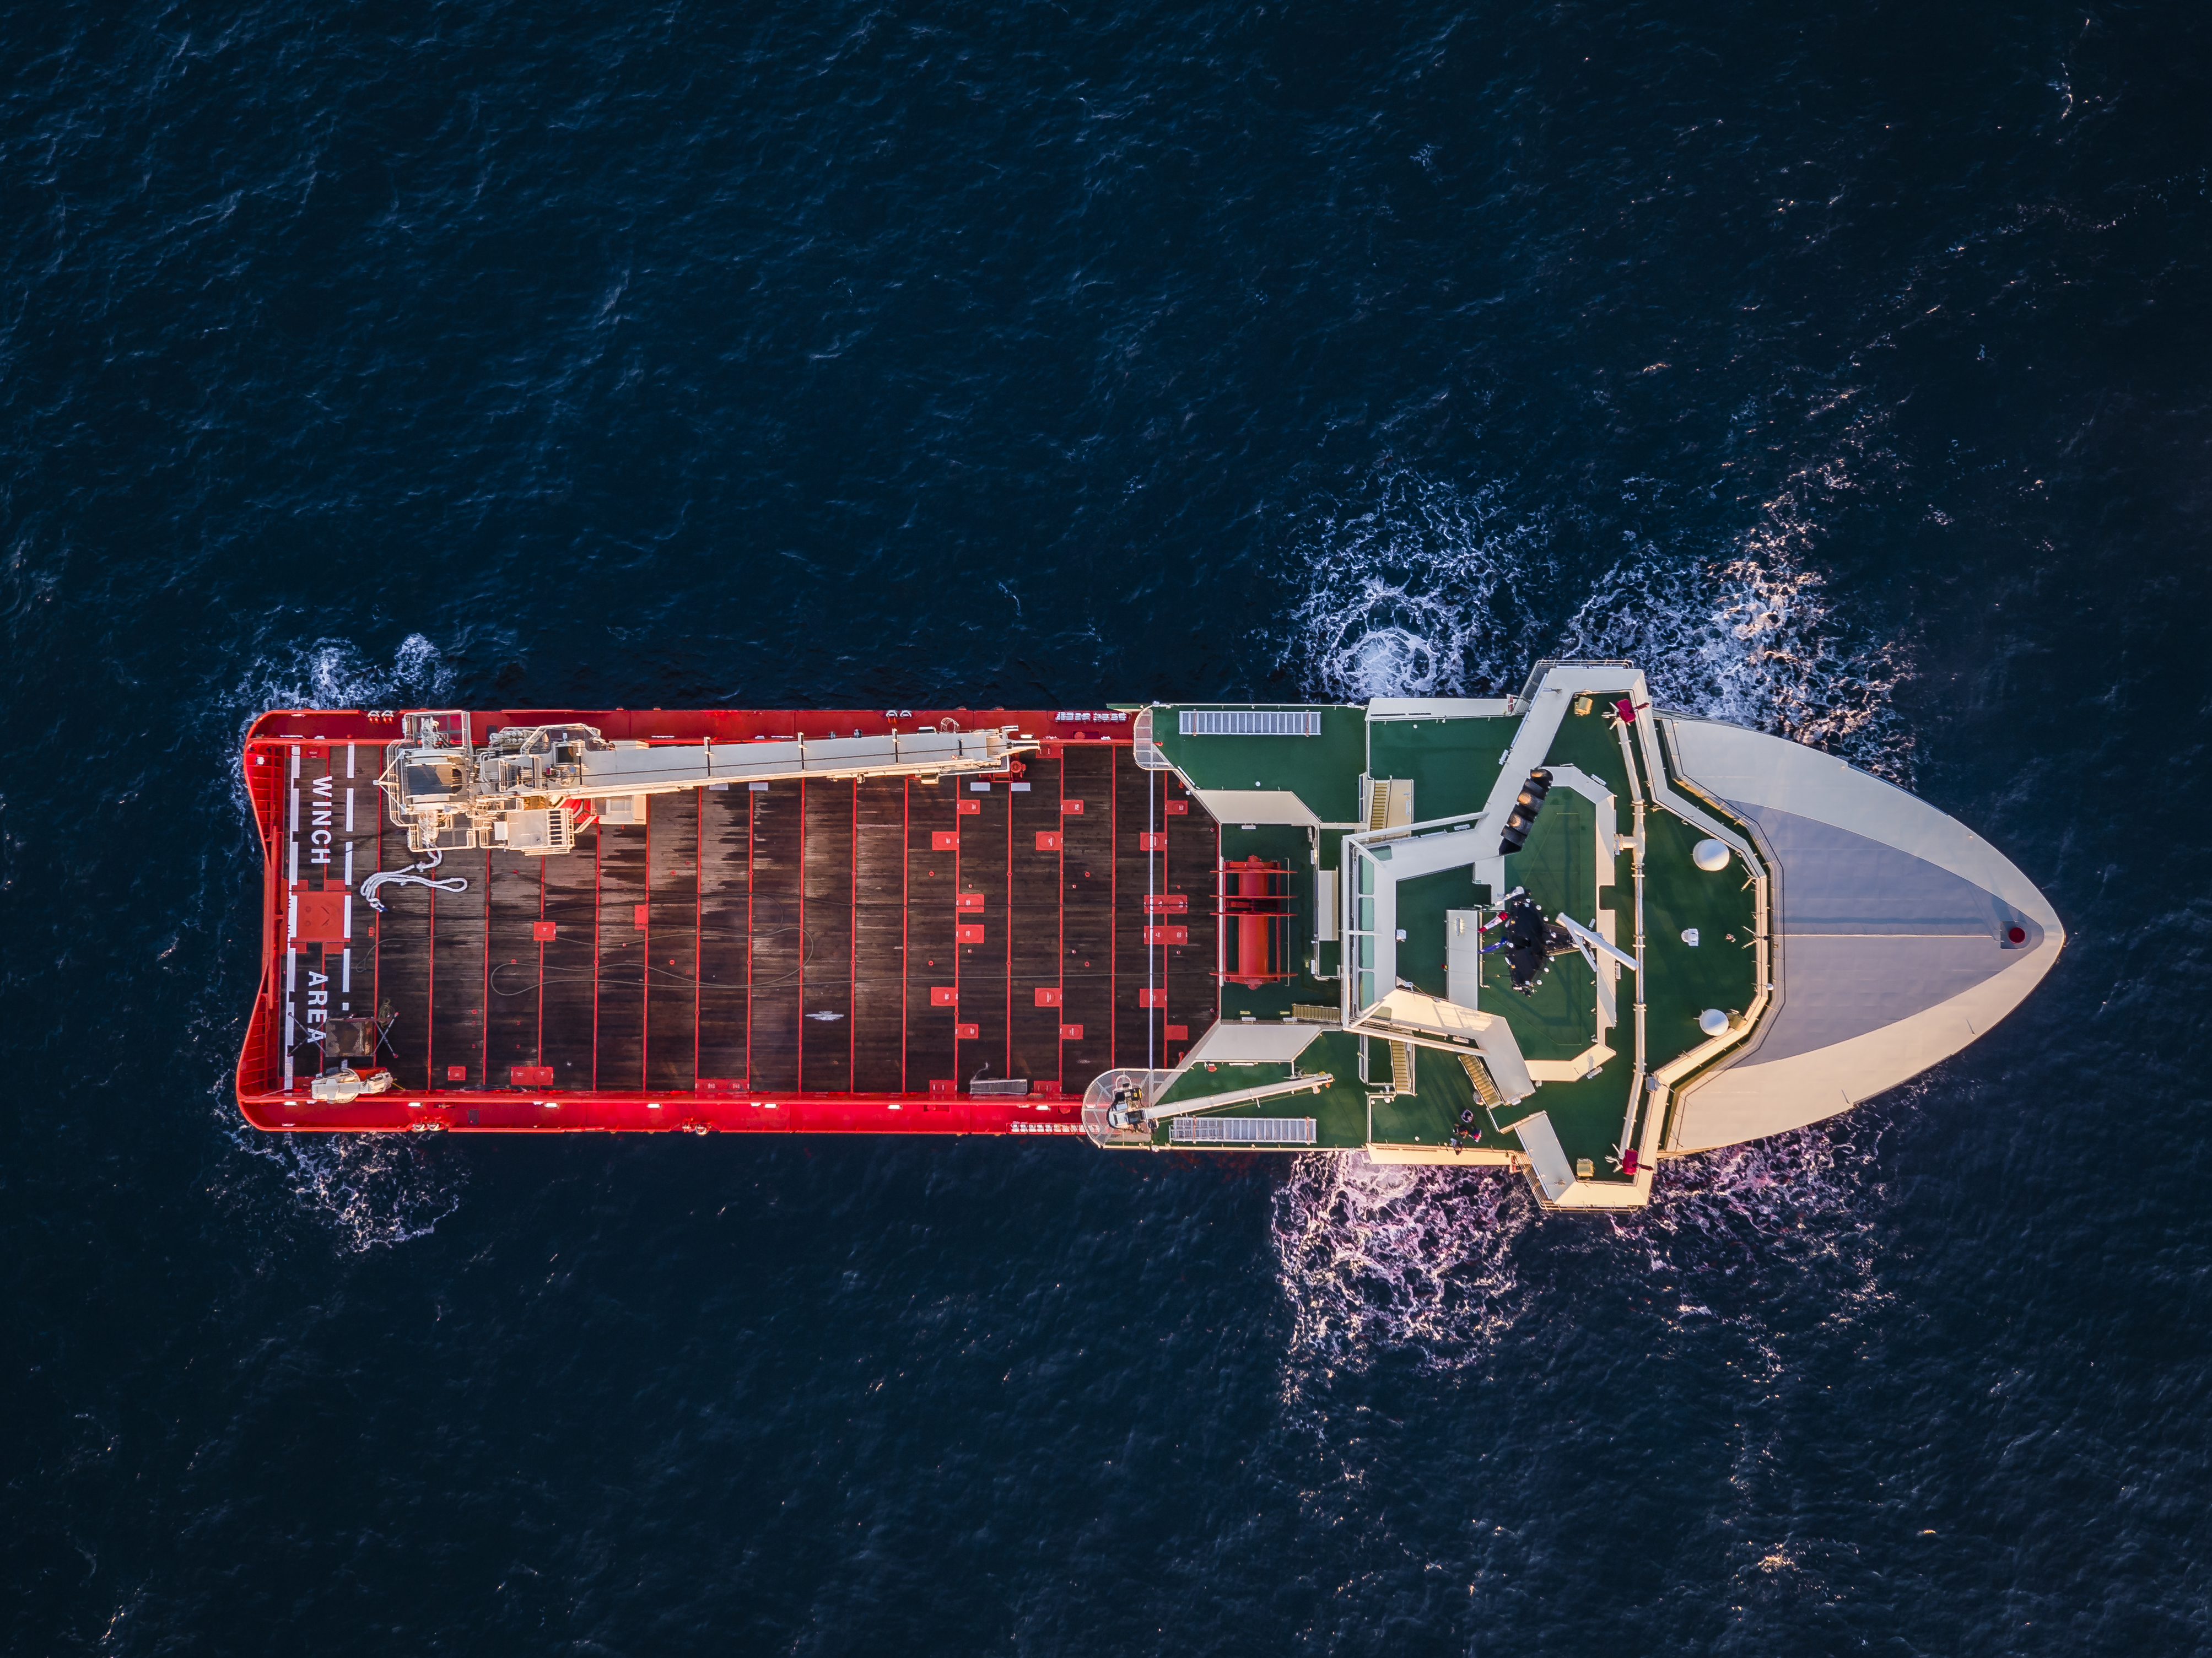
\includegraphics[width=\paperwidth, keepaspectratio]{cover_PSV_5000_top.jpg}};
		
		\node (white-glow) at (current page.center) [fill = white, minimum width = \paperwidth, minimum height = \paperheight, opacity = 0.27]{};
		
		\node (title-box) at (current page.east) [fill = lightgray, minimum width=.5\paperwidth, minimum height=7cm, fill opacity = 0.7, xshift=-.25\paperwidth, yshift=-5cm, text=white] {\Huge{\@title}};
		
		\node (grey-bar) [fill = black, minimum width=.5\paperwidth, minimum height=1cm, fill opacity = 0.5, xshift=-.25\paperwidth, xshift=.25\paperwidth, yshift = -4cm] at (title-box){};
		
		
	\end{tikzpicture}
	
	%% Create empty page for two-sided printing
	\clearpage
	\thispagestyle{empty}
	\vspace*{5cm}
	\begin{center}
		This page is intentionally left blank.
	\end{center}
	%% Title page
	\setcounter{page}{0}
	
	\title{\doctitle}
	\date{\today}
	\author{\docauthor}
	
	\maketitle
	

	
}
	